\chapter{Resultados e Discussões}

Os experimentos foram realizados com a base de dados organizada como descrita no Capítulo 4 relativo à Preparação de Dados. Os experimentos foram feitos com o apoio da ferramenta \textit{Scikit-Learn} que possui a implementação de diversos algoritmos de aprendizado de máquina e agrupamento, dentre eles K-Médias, que já foi discutido no capítulo 3. Também foi utilizado o pacote \textit{NumPy}, ferramenta para cálculos matriciais não menos importantes para o sucesso do trabalho.

Para a preparação das análises foi adicionado ao banco de dados o registro de atividades do servidor DNS do IME de 12 de março de 2012. Nesse registro de atividades há rastros de 3 suspeitos já confirmados como parte integrante de botnets, através de inspeções manuais feitas na época.

Foi realizada a comparação da qualidade da saída algoritmo para dados normalizados e não normalizados. Para normalizar, decidiu-se arbitrariamente, utilizar a forma \(\frac{\mathbf{X} - \mathbf{\bar{X}}}{\sigma} \).

\section{Análise do Número de Grupos}

Para o cálculo da distribuição da função custo, foram criados 10 modelos para cada quantidade de centroides e calculou-se a média das funções de custos dentre cada quantidade de centroide. Esse procedimento é realizado para estabilizar os valores da função custo, já que a função custo pode estar sujeita a flutuação, por outro lado isso não pareceu crítico para esse conjunto de dados.

As figuras \ref{fig:cost_per_k} e \ref{fig:cost_per_k_not_norm} apresentam o comportamento dos valores da função custo ao serem adicionados centroides.

\begin{figure}[htbp]
\centering
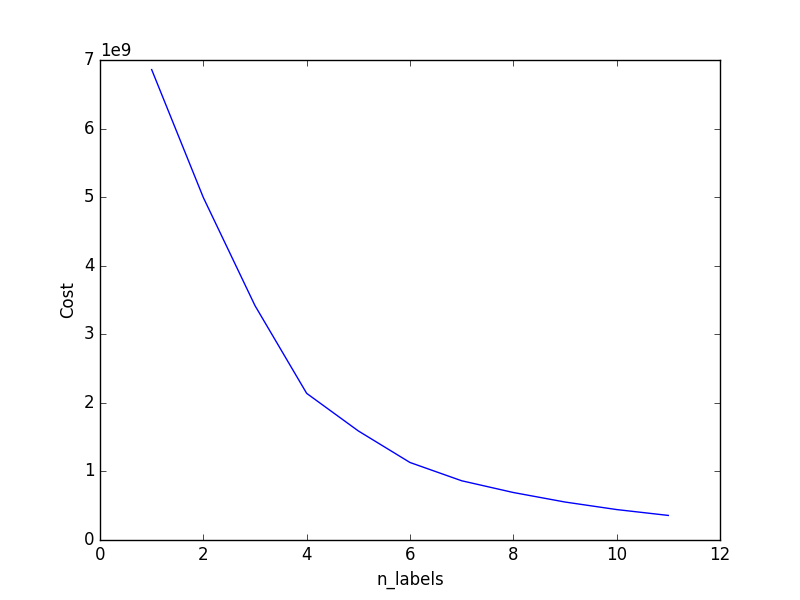
\includegraphics[scale=0.7]{cost_per_k}
\caption[Custo pelo Número de Centróides para Dados Normalizados]{Custo pelo Número de Centróides para Dados Normalizados} \label{fig:cost_per_k}
\end{figure}

\begin{figure}[htbp]
\centering
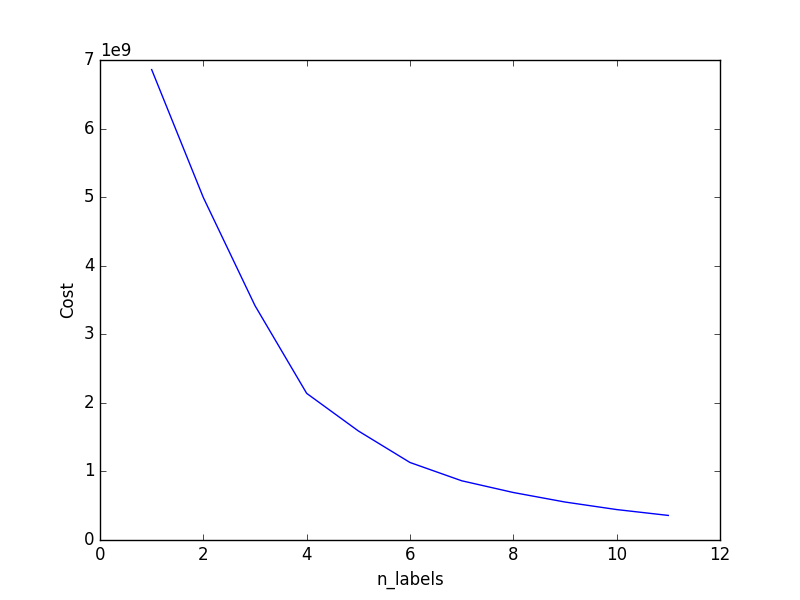
\includegraphics[scale=0.7]{cost_per_k_not_norm}
\caption[Custo pelo Número de Centróides para Dados não Normalizados]{Custo pelo Número de Centróides para Dados não Normalizados} \label{fig:cost_per_k_not_norm}
\end{figure}

Apesar de se perceber um bico quando o modelo tem 4 centroides em ambas figuras, ainda há ambiguidade quanto ao ponto crítico. Outras técnicas mais robustas serão avaliadas nas fases posteriores do projeto para validar a hipótese de que há utilização de 4 centróides gera os melhores resultados.

\section{Análise da Base de Dados}

Utilizando-se 4 centroides como parâmetro, foram realizadas análises da eficácia do algortimo de agrupamento ao conjunto de exemplos contidos no banco de dados. Em todos os experimentos o sistema consulta a tabela \textit{clients} do banco de dados e retorna na saída padrão a cardinalidade de cada grupo e os IPs das máquina no menor grupo.

A primeira análise foi realizada observando os seguintes campos:

\begin{itemize}
\item \textit{count\_domain\_with\_numbers, }
\item \textit{average\_domain\_length, }
\item \textit{std\_domain\_length, }
\item \textit{count\_request, }
\item \textit{average\_requisition\_degree, }
\item \textit{std\_requisition\_degree e }
\item \textit{minimum\_requisition\_degree }
\end{itemize}

Os dados foram fornecidos ao algoritmo sem nenhum tratamento posterior, já que os dados já foram tratados previamente. Como resultado obteve-se a saída representada na figura \ref{fig:first_out}. Esse resultado não foi considerado um sucesso, pois o menor grupo não continha nenhum dos 3 suspeitos conhecidos, porém já apresenta um grupo de cardinalidade reduzida conforme era esperado.

\begin{figure}[htbp]
\centering
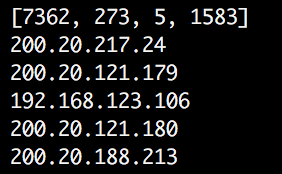
\includegraphics[scale=0.7]{first_out}
\caption[Resultado do Experimento não Normalizado]{Resultado do Experimento não Normalizado} \label{fig:first_out}
\end{figure}

Para a segunda análise, foi efetuada a normalização das características, para que cada uma tivesse o mesmo impacto para as distâncias utilizadas no algoritmo, independente do intervalo para os valores de cada uma. Após essa alteração, observou-se a saída mostrada na Figura \ref{fig:second_out}. Esse foi considerado um resultado bastante satisfatório, já que duas máquinas já confirmadas como pertencentes a botnets foram detectadas no menor grupo, cujos endereços de IP são \textit{200.213.86.2} e \textit{200.213.86.14}.

\begin{figure}[htbp]
\centering
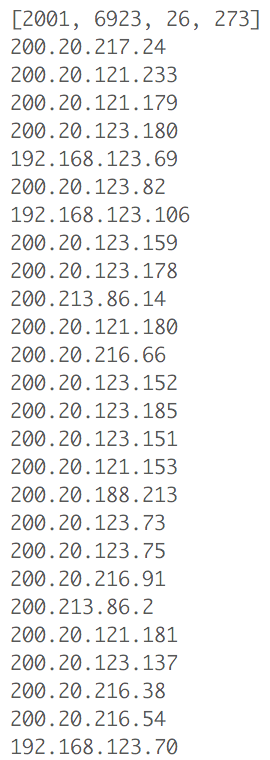
\includegraphics[scale=0.7]{second_out}
\caption[Resultado do Experimento Normalizado]{Resultado do Experimento Normalizado} \label{fig:second_out}
\end{figure}

A hipótese que se levanta para explicar o sucesso é que apesar de as máquinas com comportamento suspeito divergirem das outras máquinas, por exemplo em quantidade de requisição, a distância marginal entre elas é grande o suficiente para confundir o algoritmo ao tentar agrupa-los.

Além disso observou-se que, ao ser descartado, o campo \textit{std\_requisition\_degree} não influenciou na identificação dos itens do menor grupo, isto é os mesmo 26 elementos permanecem consistentemente no mesmo grupos. Isso reforça a necessidade de ser aplicada uma técnica para realizar a seleção das melhores características.